\documentclass[aspectratio=169,11pt]{beamer}

\usetheme{Madrid}
\usecolortheme{default}
\setbeamertemplate{navigation symbols}{}
\setbeamertemplate{footline}[frame number]

\usepackage{amsmath,amssymb}
\usepackage{graphicx}
\usepackage{tikz}
\usetikzlibrary{positioning,calc}
\usetikzlibrary{arrows.meta,decorations.pathmorphing}

\definecolor{RamRed}{RGB}{190,40,45}
\definecolor{RamBlue}{RGB}{30,90,180}
\definecolor{SoftGray}{RGB}{245,245,245}
\definecolor{DarkGray}{RGB}{70,70,70}
\definecolor{MapGreen}{RGB}{48,150,95}
\definecolor{MapGold}{RGB}{235,180,45}

\setbeamercolor{title}{fg=DarkGray}
\setbeamercolor{frametitle}{fg=white,bg=RamBlue}
\setbeamercolor{structure}{fg=RamBlue}

\tikzset{
  v/.style={circle,draw=black,fill=white,inner sep=1.8pt},
  edge/.style={draw=RamBlue,line width=1.25pt},
  topic/.style={draw=black!30,fill=SoftGray,rounded corners=5pt,inner sep=7pt,
    text width=5.8cm,minimum height=1.65cm,align=left},
}


\usepackage{booktabs}
\tikzset{dot/.style={circle,fill=black,inner sep=2pt}, lab/.style={circle,draw=black,fill=white,inner sep=2pt,minimum size=6mm,font=\small},selected/.style={draw=RamRed,line width=2pt}}

\newcommand{\Def}[2]{\begin{block}{#1}#2\end{block}}
\newcommand{\Thm}[2]{\begin{block}{#1}#2\end{block}}
\renewcommand{\Proof}[1]{\begin{block}{Proof}\normalsize #1\end{block}}
\newcommand{\Question}[1]{\begin{block}{Question}#1\end{block}}
\renewcommand{\Example}[1]{\begin{block}{Example}#1\end{block}}
\newcommand{\fall}[2]{#1^{\underline{#2}}}
\newcommand{\rise}[2]{#1^{\overline{#2}}}
\newcommand{\stir}[2]{\left\{\begin{matrix}#1\\#2\end{matrix}\right\}}
\newcommand{\cyc}[2]{\left[\begin{matrix}#1\\#2\end{matrix}\right]}
\newcommand{\eul}[2]{\left\langle\begin{matrix}#1\\#2\end{matrix}\right\rangle}
\newcommand{\coef}[2]{[#1^{#2}]}
\newcommand{\gap}{\par\medskip}

\title{Some Essential Problems}
\author{Jeremy Quastel}\date{}\begin{document}
\begin{frame}[plain]\begin{center}{\Huge\bfseries Some Essential Problems}\par\vspace{.25cm}{\Large Section 2.1}\par\vspace{.15cm}{\large Harris--Hirst--Mossinghoff, \emph{Combinatorics and Graph Theory}}\par\vspace{.1cm}\resizebox{!}{2.7cm}{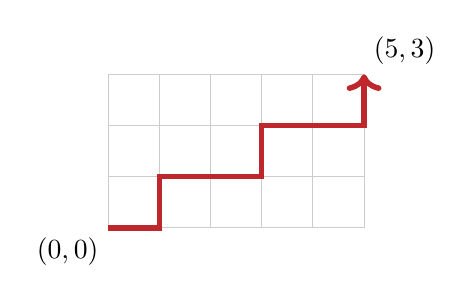
\begin{tikzpicture}[scale=.65]\draw[step=1,black!20](0,0)grid(5,3);\draw[selected,->](0,0)--(1,0)--(1,1)--(3,1)--(3,2)--(5,2)--(5,3);\node[below left]at(0,0){$(0,0)$};\node[above right]at(5,3){$(5,3)$};\end{tikzpicture}}\par\vspace{.25cm}Jeremy Quastel\end{center}\end{frame}
\begin{frame}[plain]\large \begin{center}{\Huge\bfseries Today\textquotesingle s lecture}\par\vspace{.5cm}\end{center}\begin{columns}[c,onlytextwidth]\begin{column}{.48\textwidth}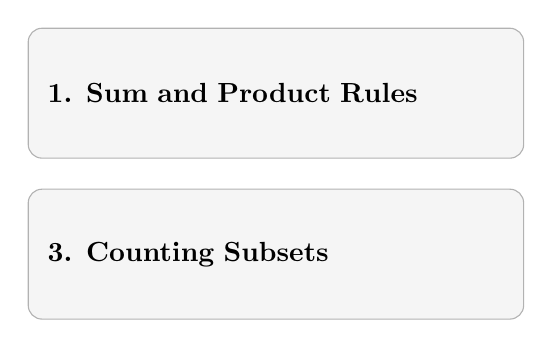
\begin{tikzpicture}\node[topic](a){\textbf{1. Sum and Product Rules}};\node[topic,below=.38cm of a]{\textbf{3. Counting Subsets}};\end{tikzpicture}\end{column}\begin{column}{.48\textwidth}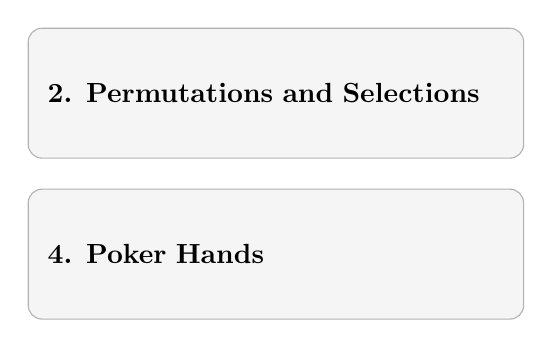
\begin{tikzpicture}\node[topic](a){\textbf{2. Permutations and Selections}};\node[topic,below=.38cm of a]{\textbf{4. Poker Hands}};\end{tikzpicture}\end{column}\end{columns}\end{frame}
\begin{frame}{What exactly are we counting?}
\large
\Question{How many ways can we choose three objects from a collection of ten?}
\gap The answer depends on the rules:
\begin{itemize}\item Does order matter?\item Can an object be used more than once?\item Are the objects distinguishable?\end{itemize}
\end{frame}
\begin{frame}{The sum rule}
\large
\Thm{Sum rule}{If a set of outcomes is partitioned into disjoint classes of sizes $a_1,\ldots,a_r$, then its size is $a_1+\cdots+a_r$.}
\Example{A committee chooses either one of $8$ first-year students or one of $6$ second-year students. There are $8+6=14$ choices.}
\end{frame}
\begin{frame}{Why disjointness matters}
\large
\Question{There are $20$ students taking algebra and $15$ taking combinatorics. How many take at least one of the courses?}
\gap Adding $20+15$ counts a student in both courses twice.
\gap The sum rule applies directly only when the classes are disjoint. We will later correct overlaps using inclusion and exclusion.
\end{frame}
\begin{frame}{The product rule}
\large
\Thm{Product rule}{Suppose a procedure has $r$ successive stages, with $a_i$ choices at stage $i$ for every possible set of earlier choices. Then there are
\[a_1a_2\cdots a_r\]
complete outcomes.}
\gap The actual choices may depend on earlier stages; their number must be the stated $a_i$.
\end{frame}
\begin{frame}{A product-rule example}
\large
\Example{How many three-digit positive integers have distinct digits?}
\gap The first digit has $9$ choices. The second has $9$ choices, including zero but excluding the first digit. The last has $8$ choices.
\[9\cdot9\cdot8=648.\]
\end{frame}
\begin{frame}{Permutations}
\large
\Def{Permutation}{A permutation of $n$ distinct objects is an ordering of all of them.}
\Thm{Counting permutations}{There are
\[n!=n(n-1)\cdots2\cdot1\]
permutations. We use $0!=1$.}
\end{frame}
\begin{frame}{Ordered selections without repetition}
\large
\Def{Falling factorial}{For $0\leq k\leq n$,
\[\fall{n}{k}=n(n-1)\cdots(n-k+1)=\frac{n!}{(n-k)!}.\]}
\gap This counts ordered selections of $k$ distinct objects from $n$ objects. In particular, $\fall{n}{0}=1$.
\end{frame}
\begin{frame}{Ordered selections with repetition}
\large
\Thm{Counting words}{The number of words of length $k$ over an alphabet of $n$ symbols is $n^k$.}
\Proof{Each of the $k$ positions has $n$ choices. Apply the product rule.}
\Example{There are $2^k$ binary words of length $k$ and $10^k$ strings of $k$ decimal digits.}
\end{frame}
\begin{frame}{Unordered selections}
\large
\Def{Binomial coefficient}{The number of $k$-element subsets of an $n$-element set is denoted by $\binom nk$.}
\Thm{Formula}{For $0\leq k\leq n$,
\[\binom nk=\frac{n!}{k!(n-k)!}.\]}
\end{frame}
\begin{frame}{Why divide by $k!$?}
\large
\Proof{There are $\fall nk$ ordered selections of $k$ distinct objects. Each $k$-element subset appears once for every ordering of its elements, hence exactly $k!$ times. Therefore
\[\binom nk=\frac{\fall nk}{k!}.\]}
\gap Division works because every desired outcome has the same number of ordered representations.
\end{frame}
\begin{frame}{Committees and officers}
\large
\Question{From $12$ people, choose a committee of $4$, and then choose a chair and secretary from that committee.}
\gap First the committee, then the officers:
\[\binom{12}{4}\cdot4\cdot3.\]
\gap First the officers, then the other members:
\[12\cdot11\binom{10}{2}.\]
\end{frame}
\begin{frame}{A first double count}
\large
\[\binom{12}{4}\cdot4\cdot3=12\cdot11\binom{10}{2}.\]
\gap Both sides count exactly the same objects in different orders.
\gap This method often proves identities more naturally than factorial manipulation.
\end{frame}
\begin{frame}{Counting all subsets}
\large
\Thm{Theorem}{An $n$-element set has $2^n$ subsets.}
\Proof{For each element, independently decide whether to include it. There are two choices for each of $n$ elements.}
\gap Grouping subsets according to size also gives
\[\sum_{k=0}^n\binom nk=2^n.\]
\end{frame}
\begin{frame}{Selections with repetition}
\large
\Question{How many ways are there to choose $k$ objects from $n$ types when repetition is allowed and order does not matter?}
\gap An outcome is specified by nonnegative integers
\[x_1+\cdots+x_n=k.\]
\gap We will derive $\binom{n+k-1}{k}$ using stars and bars and generating functions.
\end{frame}
\begin{frame}{Four basic models}
\large
\begin{center}\renewcommand{\arraystretch}{1.65}
\begin{tabular}{lcc}
& No repetition & Repetition allowed\\\hline
Ordered & $\dfrac{n!}{(n-k)!}$ & $n^k$\\
Unordered & $\binom nk$ & $\binom{n+k-1}{k}$
\end{tabular}\end{center}
\gap Here the $n$ available objects or types are distinguishable.
\end{frame}
\begin{frame}{Circular arrangements}
\large
\Thm{Theorem}{There are $(n-1)!$ circular arrangements of $n$ distinct people, when rotations are identified and reflections are different.}
\Proof{Fix one specified person in a reference seat. Arrange the remaining $n-1$ people around the circle.}
\gap Changing the equivalence rule changes the counting problem.
\end{frame}
\begin{frame}{Lattice paths}
\large
\begin{center}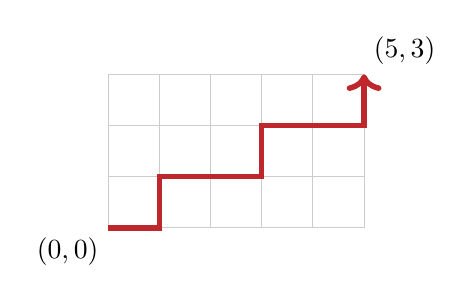
\begin{tikzpicture}[scale=.65]\draw[step=1,black!20](0,0)grid(5,3);\draw[selected,->](0,0)--(1,0)--(1,1)--(3,1)--(3,2)--(5,2)--(5,3);\node[below left]at(0,0){$(0,0)$};\node[above right]at(5,3){$(5,3)$};\end{tikzpicture}\end{center}
\Question{How many paths from $(0,0)$ to $(5,3)$ use only right and up steps?}
\end{frame}
\begin{frame}{Encoding a path}
\large
\Proof{Every path has $5$ right steps and $3$ up steps. Choose the $3$ positions occupied by up steps among the $8$ steps:
\[\binom83=56.\]}
\gap In general, the number of such paths to $(a,b)$ is $\binom{a+b}{a}$.
\end{frame}
\begin{frame}{Counting by complements}
\large
\Example{How many binary words of length $10$ contain at least one $1$?}
\gap There are $2^{10}$ words in total. Exactly one, the all-zero word, has no $1$.
\[2^{10}-1=1023.\]
\gap A difficult positive condition can have a simple complement.
\end{frame}
\begin{frame}{Poker hands}
\large
\Def{The model}{A standard deck has $52$ distinct cards: $13$ ranks and $4$ suits. A poker hand is an unordered set of $5$ cards.}
\gap The total number of hands is
\[\binom{52}{5}=2,598,960.\]
\end{frame}
\begin{frame}{Four of a kind}
\large
\Example{Choose a hand with four cards of one rank and a fifth card of a different rank.}
\gap Choose the repeated rank in $13$ ways. All four suits are forced. Choose the fifth card from the $48$ cards of other ranks.
\[13\cdot48=624.\]
\end{frame}
\begin{frame}{Full houses}
\large
\Example{A full house has three cards of one rank and two of another rank.}
\gap Choose the triple rank, its suits, the pair rank, and its suits:
\[13\binom43\cdot12\binom42=3744.\]
\gap The two ranks have different roles, so they are chosen in order.
\end{frame}
\begin{frame}{Exactly one pair}
\large
\normalsize
Choose the pair rank and its two suits. Choose three distinct other ranks, and one suit for each:
\[13\binom42\binom{12}{3}4^3=1,098,240.\]
\gap The requirement that the other ranks be distinct excludes two pairs, three of a kind, and full houses.
\gap Choosing three arbitrary cards after choosing the pair would overcount and include unwanted hands.
\end{frame}
\begin{frame}{Flushes}
\large
\Example{A hand all of whose cards have the same suit can be chosen in
\[4\binom{13}{5}=5148\]
ways.}
\gap This includes straight flushes. Under the usual poker classification, exclude the $10$ consecutive rank patterns in each of $4$ suits:
\[5148-40=5108.\]
\end{frame}
\begin{frame}{Practice}
\large
\Question{How many $5$-element subsets of $\{1,\ldots,12\}$ contain exactly two elements of $\{1,2,3,4\}$?}
\gap Identify two independent choices before calculating.
\end{frame}
\begin{frame}{Practice: solution}
\large
\Proof{Choose $2$ of the first $4$ elements and $3$ of the remaining $8$:
\[\binom42\binom83=6\cdot56=336.\]
The two choices determine the subset uniquely.}
\end{frame}
\begin{frame}{Summary}
\large
\begin{itemize}
\item Use the sum rule for disjoint alternatives and the product rule for successive choices.
\item Specify whether order and repetition matter.
\item Divide only when every outcome has the same multiplicity.
\item Encode objects as words, subsets, or paths whenever possible.
\end{itemize}
\end{frame}
\begin{frame}{Next time: Binomial Coefficients}\begin{center}{\Huge Binomial Coefficients}\end{center}\end{frame}
\end{document}